\documentclass[titlepage]{article}
% \usepackage[margin=2.5cm]{geometry}
\usepackage[margin=2.5cm, headheight=0pt, headsep=1cm]{geometry}
\usepackage{enumerate, fancyhdr, graphicx, amsmath, nth}
\usepackage[binary-units=true]{siunitx}

\title{Hurricane Evacuation Strategies for the State of Mississippi}
\author{Paul Chesnais (pmc85), Antoine Pourchet (app63), and Ryan Vogan (rcv39)\\2015 Cornell Mathematical Contest in Modeling}
\date{November 16, 2015}

\pagestyle{fancy}
\fancyhead{}
\lhead{Chesnais, Pourchet, Vogan}
\chead{Hurricane Evacuation Strategies}
\rhead{November 16, 2015}
\fancyfoot{}
\rfoot{\thepage}
\renewcommand{\headrulewidth}{0.5pt}
\renewcommand{\footrulewidth}{0.5pt}

\usepackage{listings, color, times, textcomp, float, hyperref, setspace, subcaption}
\definecolor{Code}{rgb}{0,0,0}
\definecolor{Decorators}{rgb}{0.5,0.5,0.5}
\definecolor{Numbers}{rgb}{0.5,0,0}
\definecolor{MatchingBrackets}{rgb}{0.25,0.5,0.5}
\definecolor{Keywords}{rgb}{0,0,1}
\definecolor{self}{rgb}{0,0,0}
\definecolor{Strings}{rgb}{0,0.63,0}
\definecolor{Comments}{rgb}{0,0.63,1}
\definecolor{Backquotes}{rgb}{0,0,0}
\definecolor{Classname}{rgb}{0,0,0}
\definecolor{FunctionName}{rgb}{0,0,0}
\definecolor{Operators}{rgb}{0,0,0}
\definecolor{Background}{rgb}{0.98,0.98,0.98}
\definecolor{mygreen}{RGB}{28,172,0}
\definecolor{mylilas}{RGB}{170,55,241}

\lstdefinestyle{Python}{
  backgroundcolor=\color{Background},basicstyle=\ttfamily\small\setstretch{1},breaklines=true,
  commentstyle=\color{Comments}\slshape,emph={self},emphstyle={\color{self}\slshape},frame=l,framexbottommargin=2em,
  framextopmargin=2em,keywordstyle={[2]\color{Decorators}\slshape},keywordstyle={\color{Keywords}\bfseries},
  language=Python,morecomment=[s][\color{Strings}]{"""}{"""},morecomment=[s][\color{Strings}]{'''}{'''},
  morekeywords={[2]@invariant},morekeywords={import,from,class,def,for,while,if,is,in,elif,else,not,and,or,print,break,
  continue,return,True,False,None,access,as,del,except,exec,finally,global,import,lambda,pass,print,raise,try,assert},
  numbers=left,numbersep=1em,numberstyle=\footnotesize,showspaces=false,showstringspaces=false,showtabs=false,
  stringstyle=\color{Strings},tabsize=4,xleftmargin=1em,
}

\lstdefinestyle{Matlab}{
  backgroundcolor=\color{Background},basicstyle=\ttfamily\small\setstretch{1},breaklines=true,
  commentstyle=\color{mygreen},emph=[1]{for,end,break},emphstyle=[1]\color{red},frame=l,identifierstyle=\color{black},
  keywordstyle=[2]{\color{black}},keywordstyle=\color{blue},language=Matlab,literate={~} {\texttildelow}{1},
  morekeywords=[2]{1},morekeywords={matlab2tikz},numbers=left,numbersep=9pt,numberstyle={\tiny \color{black}},
  showstringspaces=false,stringstyle=\color{mylilas},
}

\begin{document}
\maketitle
\thispagestyle{empty}

\section{Executive Summary}
\label{sec:summary}

\section{Introduction}
\label{sec:introduction}
  The Mississippi Emergency Management Administration (MSEMA) has hired our team to design evacuation routes for at-risk counties in the coastal regions of southern Mississippi. Given that this coastal area is a strong commercial center, the govermental authorities want to minimize the number of unnecessary evacuations. Under this requirement, it is more advantageous to withhold ordering an evacuation for as long as possible. The reasons for this are two-fold. First, this ensures that local businesses can remain open for as long as possible. Second, this ensures that the forecasting reports at the time of the evacuation order are as accurate as possible. Therefore, our models seek to recommend an optimal evacuation plan as well as the latest possible time at which it is safe to enact this plan.

\section{Model Assumptions}
\label{sec:assumptions}
  The MSEMA specified that our plan should be enacted on a per-county basis. As you can see in the following figure, these counties are approximately equally sized:
  \begin{figure}[H]
  \centering
  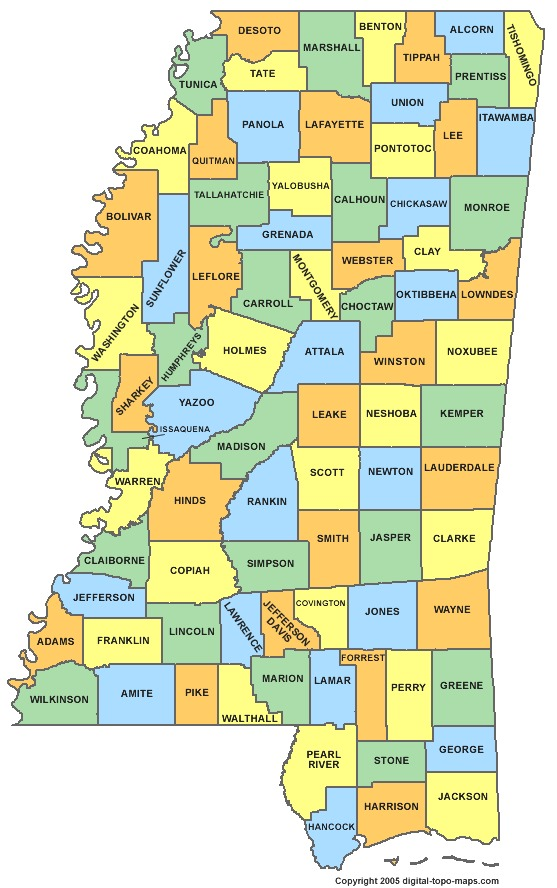
\includegraphics[width=.5\textwidth]{figures/county_map.jpg}
  \caption{A Map of Counties in the State of Mississippi \cite{county_map}}
  \end{figure}
  As a result of this, we assume that each county can be modeled as a single node in a bidirected graph. Here an edge from node $i$ to node $j$ represents that a refugee can directly reach county $j$ from county $i$. Therefore, we constructed our network of Mississippi counties by connecting a county's node to the nodes of all bordering counties. This produced the following graph:




\section{Statical Analysis of Historical Hurricane Data}
\label{sec:hurricanes}


\section{Markov Process Analysis of Strictly Northern Evacuations}
\label{sec:markov}
  \subsection{Model Description}
  \subsection{Parameter Values and Justification}
  \subsection{Results}
  \subsection{Strengths and Weaknesses}

\section{Maximum Flow Analysis of Strictly Northern Evacuations}
\label{sec:maxflow}
  \subsection{Model Description}
  \subsection{Parameter Values and Justification}
  \subsection{Results}
  \subsection{Strengths and Weaknesses}

\section{Stochastic Model of Landfall-Avodiant Evacuations}
\label{sec:stochastic}
  \subsection{Model Description}

  \subsection{Parameter Values and Justification}
  \subsection{Results}
  \begin{figure}
    \center
    \begin{subfigure}[b]{0.5\textwidth}
      \center
      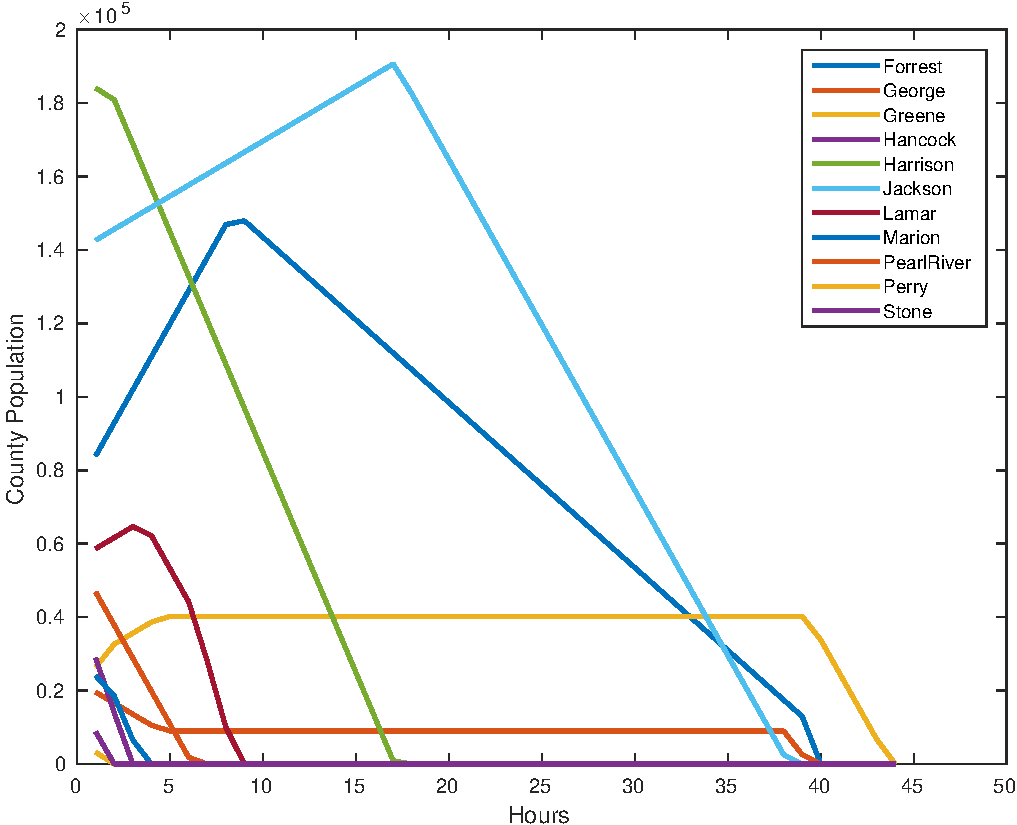
\includegraphics[width=\linewidth]{figures/pred_hancock-crop.pdf}
      \caption{Predicted Evacuation for Landfall in Hancock County}
    \end{subfigure}~
    \begin{subfigure}[b]{0.5\textwidth}
      \center
      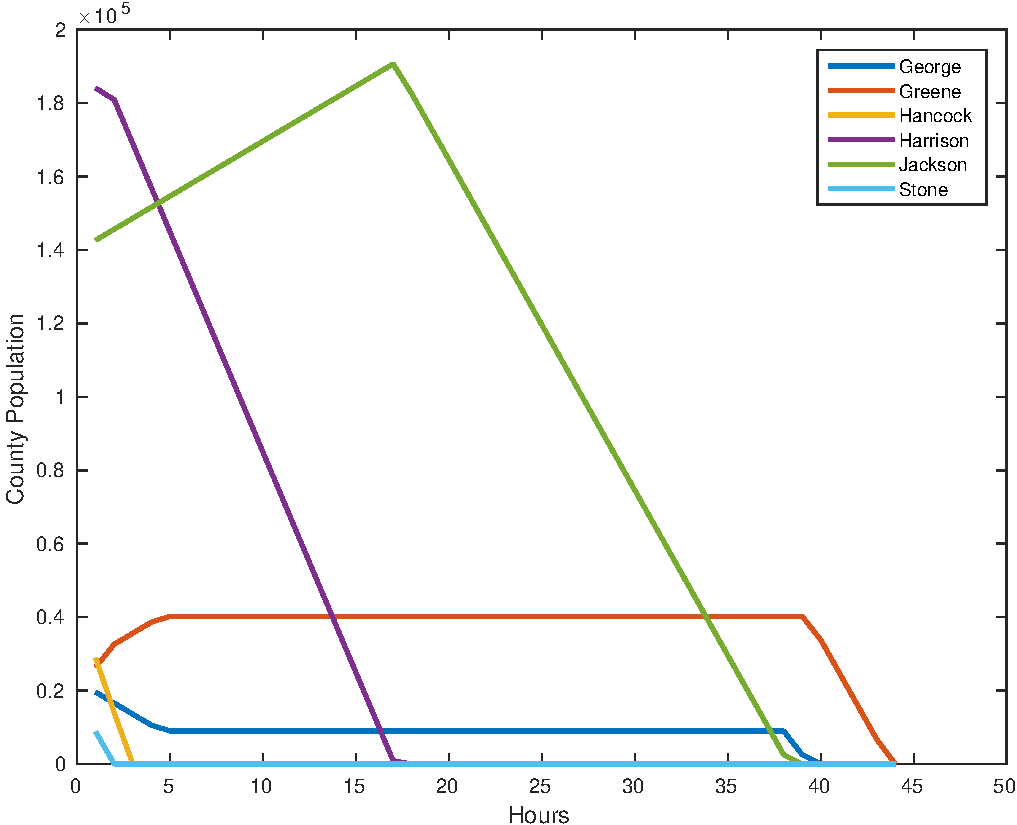
\includegraphics[width=\linewidth]{figures/pred_jackson-crop.pdf}
      \caption{Predicted Evacuation for Landfall in Jackson County}
    \end{subfigure}
    \caption{}
  \end{figure}
  \subsection{Strengths and Weaknesses}

\section{Conclusions}
\label{sec:conclusions}

\section{Future Work}
\label{sec:future}

\section{Individual Contributions}
\label{sec:contributions}
  \begin{thebibliography}{9}
    \bibitem{county_map}
      \url{http://www.madeinmississippi.us/wp-content/uploads/2015/02/mississippi-county-map.jpg}
    \bibitem{pmc}
      \url{http://www.ncbi.nlm.nih.gov/pmc/articles/PMC4060166/}
    \bibitem{ms_highways}
      \url{https://www.mississippi.org/assets/docs/library/ms_highways.pdf}
  \end{thebibliography}

\end{document}